
% This work is licensed under the Creative Commons Attribution-Share Alike 2.0 France License.
% To view a copy of this license, visit http://creativecommons.org/licenses/by-sa/2.0/fr/legalcode
% or send a letter to Creative Commons, 171 Second Street, Suite 300, San Francisco, California, 94105, USA.




\chapter{Tortues à profusion\label{chap:tortue2}}
\section{Le retour de la tortue}
Revenons au module tortue que nous avions commencé à examiner au \autoref{chap:tortue1} page \pageref{chap:tortue1}. Nous allons examiner tout un ensemble de fonctions du module turtle. 

Vous vous demandez peut-être comment avoir des informations sur toutes ces commandes, en fait Python inclut une aide interne (sans parler de l'aide disponible dans le menu démarrer). Vous pouvez faire « \texttt{dir(turtle)} » pour avoir la liste de toutes les commandes inclues dans turtle. La commande « \texttt{dir} » est disponible pour tous les modules. De plus les modules bien développés incluent une aide en ligne par exemple « \texttt{help(turtle.Pen())} ». Cette aide est en anglais, malheureusement pour les francophones. Néanmoins, cela pourrait être pire dans une langue dont vous  ne comprendriez même pas les caractères. Vous pouvez essayer ces commandes dans la console ou le shell:

\begin{Verbatim}[frame=single,rulecolor=\color{mbleu}, label=à taper]
>>> dir(str)
>>> help(str.isalpha)
>>> import turtle
>>> dir(turtle)
>>> help(turtle.Pen)
\end{Verbatim}

Pour information, la méthode « \texttt{isalpha} » teste une chaîne pour savoir si elle est composée de lettres uniquement et renvoie vrai (\texttt{True}) ou faux (\texttt{False}).

Revenons, à  nouveau, sur le module « \texttt{turtle} ». Rappelez-vous, pour afficher une zone de dessin et dessiner dessus, nous avions besoin d'importer le module « \texttt{turtle} » et de créer un objet « \texttt{Pen} »:
\begin{Verbatim}[frame=single,rulecolor=\color{gray}, label=ne pas saisir]
>>> import turtle
>>> tortue = turtle.Pen()
\end{Verbatim}

À l'époque nous fermions la fenêtre en lançant « \texttt{turtle.bye()} ».

Maintenant que nous savons utiliser IDLE pour créer, exécuter et sauvegarder des programmes nous ne souhaitons pas ouvrir une  fenêtre de dessins a chaque exécution, la commande « \texttt{turtle.bye()} » permettrait de fermer la fenêtre dessin mais nous ne verrions plus le résultat de nos programmes c'est pourquoi je vous propose d'utiliser 
la méthode « \texttt{turtle.exitonclick} »  (\emph{exit} signifie sortie, \emph{on} signifie sur, \emph{click} signifie clic).

N'oubliez pas de créer une nouvelle fenêtre (\emph{new windows} dans le menu « \texttt{File} » d'IDLE ou de rouvrir un programme existant pour taper votre code.

\begin{Verbatim}[frame=single,rulecolor=\color{mbleu}, label=à taper]
import turtle
tortue = turtle.Pen()
tortue.forward(100)
turtle.exitonclick
\end{Verbatim}

Lancez le programme (sauvez le sous le nom de votre choix finissant par « \texttt{.py} » si nécessaire) puis cliquez sur la fenêtre de dessin pour quitter le programme.

Nous pouvons maintenant utiliser des fonctions simples pour déplacer notre tortue sur le zone de dessin et dessiner des formes simples. Mais encore plus intéressant nous pouvons utiliser ce que nous avons appris dans les chapitres précédents. Par exemple, le code que nous avions utilisé pour créer un carré était:

\begin{Verbatim}[frame=single,rulecolor=\color{gray}, label=ne pas saisir]
>>> tortue.forward(50)
>>> tortue.left(90)
>>> tortue.forward(50)
>>> tortue.left(90)
>>> tortue.forward(50)
>>> tortue.left(90)
\end{Verbatim}

Nous pouvons maintenant le ressaisir en utilisant un itérateur:

\begin{Verbatim}[frame=single,rulecolor=\color{mbleu}, label=à taper]
import turtle
tortue = turtle.Pen()
for x in range(4):
    tortue.forward(50)
    tortue.left(90)
    
turtle.exitonclick
\end{Verbatim}

Ce qui fait nettement moins à saisir, mais nous pouvons maintenant faire des choses un peu plus intéressantes. Essayez donc ce qui suit:
\begin{Verbatim}[frame=single,rulecolor=\color{mbleu}, label=à taper]
import turtle
tortue = turtle.Pen()
for x in range(8):
    tortue.forward(100)
    tortue.left(225)
    
turtle.exitonclick()
\end{Verbatim}

Ce code produit une étoile à huit branches comme montré sur la \autoref{fig:etoile8} (la tortue tourne de 225 degrés puis avance de 100 pixels, huit fois).
\begin{figure}[h!]
\centering
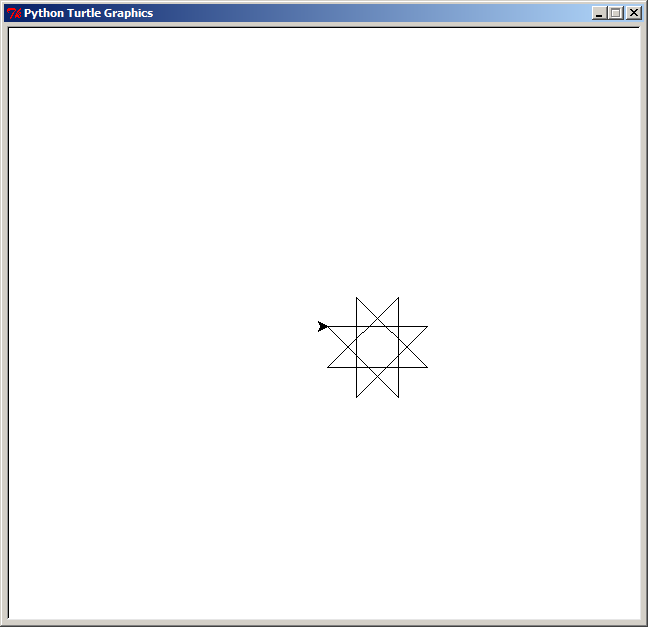
\includegraphics[scale=0.4]{images/etoile8}
\caption{Étoile à huit branches}\label{fig:etoile8}
\end{figure}


\section{Je jure [...] de dire \emph{toute} la vérité, rien que la vérité}

Comme nous avons pu le remarquer la tortue est lente, très lente... En fait on peut choisir la vitesse de la « tortue » avec la fonction « \texttt{turtle.speed} » (\emph{speed} signifie vitesse en anglais). La fonction « \texttt{turtle.speed} » prend en paramètre un entier entre zéro et dix. D'après le manuel, la vitesse de dessin va de très lent pour un, à très rapide pour dix. La vitesse normale (par défaut) est six. Pour une valeur de zéro aucune animation n'a lieu, c'est à dire que l'affichage du résultat est presque instantané:

\begin{Verbatim}[frame=single,rulecolor=\color{mbleu}, label=à taper]
import turtle
turtle.speed(0)
tortue = turtle.Pen()

for x in range(36):
    tortue.forward(200)
    tortue.left(170)
    
turtle.exitonclick()
\end{Verbatim}

Comme vous pouver le voir sur la \autoref{fig:etoile36} on obtient une étoile avec plein de branches.
\begin{figure}[h!]
\centering
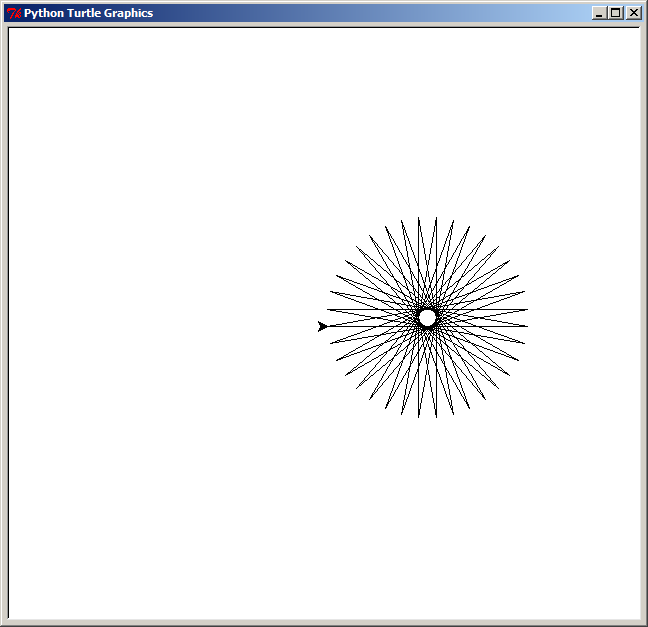
\includegraphics[scale=0.4]{images/etoile36}
\caption{Étoile à trente six branches}\label{fig:etoile36}
\end{figure}

À ce point, deux choses ont pu vous surprendre:
\begin{itemize}
\item la vitesse la plus rapide est assez lente;
\item une flèche est apparue au début du dessin lors du lancement de l'instruction\\
« \texttt{turtle.speed} ». 
\end{itemize}

En fait, il y a deux expplications à ces constatations. Le système d'affichage interne de « \texttt{turtle} » est lent, le terme instantané est donc très faux. Deuxièmement, l'instruction « \texttt{turtle.Pen()} » ne crée que par effet de bord une zone d'affichage. Cette instruction crée un stylo qui va écrire sur la zone de dessin. Si celle-ci n'existe pas, cette zone est alors créée au passage. Inversement le module « \texttt{turtle} » inclut un stylo par défaut et « \texttt{turtle.forward} » créera un stylo pour réaliser une écriture.

Malheureusement l'instruction « \texttt{turtle} » crée aussi un stylo... Heureusement il existe des instructions pour cacher ou faire apparaître les stylos.

\begin{Verbatim}[frame=single,rulecolor=\color{mbleu}, label=à taper]
import turtle
turtle.hideturtle()
turtle.speed(0)

tortue = turtle.Pen()
tortue.hideturtle()


for x in range(36):
    tortue.forward(200)
    turtle.speed(0)
    tortue.left(170)

tortue.showturtle()    
turtle.exitonclick()
\end{Verbatim}

L'instruction « \texttt{turtle.hideturtle()} » cache le stylo par défaut (\emph{hide} cacher en anglais) plus généralement si une « \texttt{variable} »  est de type « \texttt{Pen} » on peut cacher ce stylo avec « \texttt{variable.hideturtle()} ». Il est possible de cacher le stylo par défaut. S'il n'existe pas encore, il est créé caché et ne sera jamais visible sauf si nous décidons de l'afficher avec « \texttt{showturle} ». L'instruction  « \texttt{showturtle} » est généralement utilisée avant de dessiner et l'instruction « \texttt{hideturtle} » après avoir dessiné.

Par exemple on peut faire:
\begin{Verbatim}[frame=single,rulecolor=\color{mbleu}, label=à taper]
import turtle
turtle.hideturtle()
turtle.speed(0)

listestylos=[]

for x in range(36):
    listestylos.append(turtle.Pen())
    
for stylo in enumerate(listestylos): 
    stylo[1].left(10*stylo[0])
    stylo[1].forward(10*(stylo[0]+1))
    stylo[1].hideturtle()

turtle.exitonclick()
\end{Verbatim}

Dans cet exemple nous créons une liste de trente six stylos puis nous les utilisons et enfin nous les cachons.
Plusieurs remarques concernant ce code peuvent être faites:
\begin{itemize}
\item nous ajoutons des éléments sur une liste vide;
\item nous utilisons la fonction « \texttt{enumerate} ».
\end{itemize}

Pour pouvoir ajouter avec « \texttt{append} » des éléments à une liste, il est nécessaire que la liste existe au préalable, c'est pourquoi nous l'initialisons avec une liste vide « \texttt{[]} ».

La fonction « \texttt{enumerate} »  (énumérer en anglais) est utilisée pour générer des couples index et valeur (n-uplet de deux éléments) pour l'itérateur. Cette construction permet de faire un code lisible, au lieu de créer une variable artificielle et inutile « \texttt{x} »  utilisée dans un code moche:

\begin{Verbatim}[frame=single,rulecolor=\color{gray}, label=moche]
for x in range(len(listestylos)): 
    listestylos[x].left(10*x)
    listestylos[x].forward(10*(x+1))
    listestylos[x].hideturtle()
\end{Verbatim}

La fonction « \texttt{enumerate} » fournit à chaque pas un couple « \texttt{index, valeur} ». Dans notre cas l'index dans « \texttt{stylo[0]} » varie entre zéro et trente-cinq, la valeur dans « \texttt{stylo[1]} » est de type « \texttt{Pen} » et correspond aux trente six stylos que nous avions créé dans le premier itérateur.

L'abbréviation « \texttt{len} » est utilisée à la place de \emph{length} qui signifie longueur (de la liste dans notre cas).

\begin{figure}[h!]
\centering
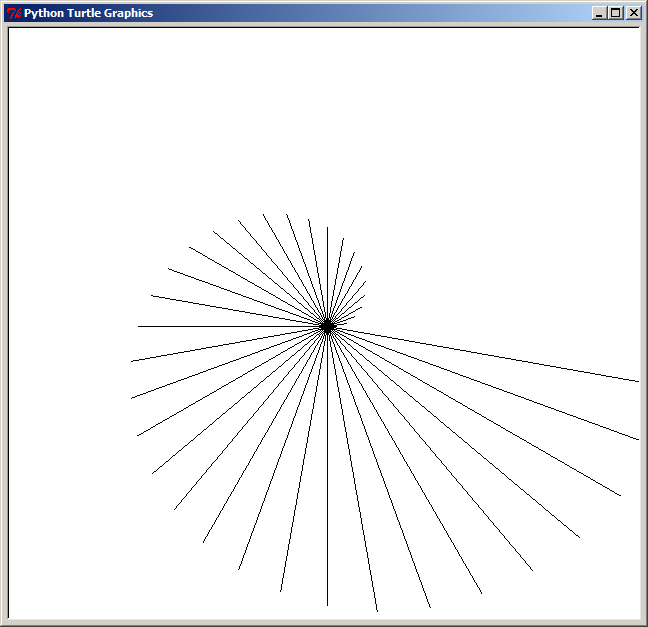
\includegraphics[scale=0.4]{images/escargot}
\caption{Escargot réalisé avec 36 stylos}\label{fig:escargot}
\end{figure}

Pour la dernière fois nous indiquons ci-dessous la totalité du code du programme: Par la suite nous indiquerons uniquement le code qui nécessite votre attention:
\begin{Verbatim}[frame=single,rulecolor=\color{mbleu}, label=ne sera plus rappelé]
import turtle
turtle.hideturtle()
turtle.speed(0)
tortue = turtle.Pen()
\end{Verbatim}
\begin{Verbatim}[frame=single,rulecolor=\color{mbleu}, label= à taper]
for x in range(1,24):
	tortue.forward(200)
	tortue.left(94)
\end{Verbatim}
\begin{Verbatim}[frame=single,rulecolor=\color{mbleu}, label=ne sera plus rappelé]
tortue.hideturtle()
turtle.exitonclick()
\end{Verbatim}
 
Ce qui donne une jolie étoile présentée \autoref{fig:etoile24}.
\begin{figure}[H]
\centering
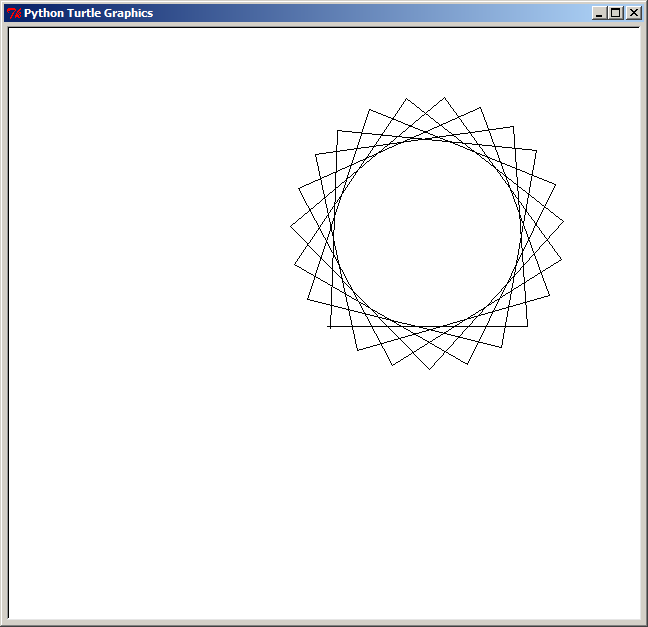
\includegraphics[scale=0.4]{images/etoile24}
\caption{Étoile à 24 branches}\label{fig:etoile24}
\end{figure}

Maintenant quelque chose d'un peu plus compliqué... Nous n'avons pas décrit tous les opérateurs. Un opérateur fort utile est « \texttt{\%} » qui est le reste d'une division entière. C'est à dire ce qui reste dans une division, avant de s'embêter avec les virgules. Cet opérateur est appelé \emph{modulo}. Si vous n'avez pas encore vu la division en classe retenez juste que si le résultat de cette opération entre deux nombres est nul, c'est que le premier nombre est divisible par le premier.

Dans notre cas nous voulons savoir si « \texttt{x} »  est pair (divisible par deux) pour une liste d'entiers successifs entre un et dix neuf:

\begin{Verbatim}[frame=single,rulecolor=\color{mbleu}, label=à taper]
for x in range(1,19):
    tortue.forward(100)
    if x % 2 == 0:
        tortue.left(175)
    else:
        tortue.left(225)
\end{Verbatim}

Le résultat de ce code est une étoile à neuf branches que vous pouvez observer sur la \autoref{fig:etoile9}.

\begin{figure}[H]
\centering
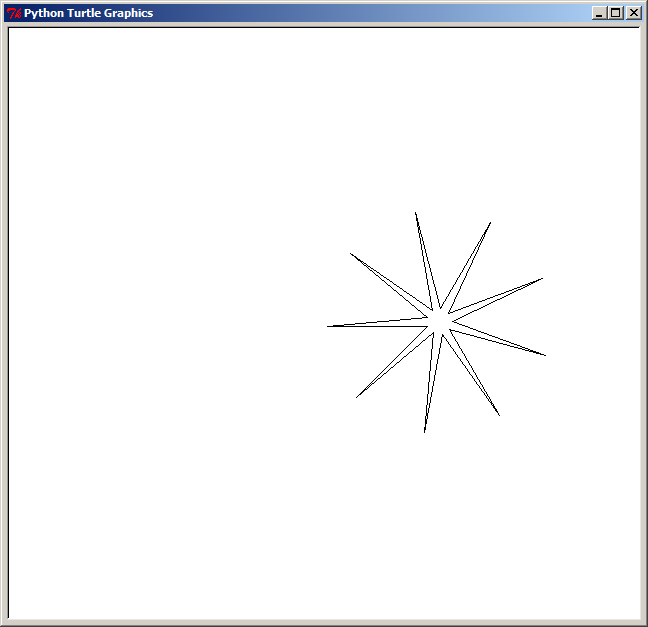
\includegraphics[scale=0.4]{images/etoile9}
\caption{Étoile à neuf branches}\label{fig:etoile9}
\end{figure}

Nous ne sommes pas obligé de nous limiter à tracer des étoiles et des formes simples. Si nous utilisons une combinaison d'appels à des fonctions, notre tortue peut dessiner différentes choses. Nous pouvons par exemple dessiner une voiture:

\begin{Verbatim}[frame=single,rulecolor=\color{mbleu}, label=à copier-coller depuis le fichier du livre]
tortue.color(1,0,0)   #color (couleur) en (rouge,vert,bleu)
tortue.begin_fill()   #begin (commencer) fill (remplir)
tortue.forward(100)
tortue.left(90)
tortue.forward(20)
tortue.left(90)
tortue.forward(20)
tortue.right(90)
tortue.forward(20)
tortue.left(90)
tortue.forward(60)
tortue.left(90)
tortue.forward(20)
tortue.right(90)
tortue.forward(20)
tortue.left(90)
tortue.forward(20)
tortue.end_fill()     #end (finir) fill (remplir)
tortue.color(0,0,0)   #(rouge,vert,bleu) entre 0 (foncé) et 1 (clair)
tortue.up()
tortue.forward(10)
tortue.down()
tortue.begin_fill()
tortue.circle(10)     #cercle de diamètre 10 pixels
tortue.end_fill()
tortue.setheading(0)  #set (fixer) heading (orientation)
tortue.up()
tortue.forward(90)
tortue.right(90)
tortue.forward(10)
tortue.setheading(0)  #orientation=0 direction initiale
tortue.begin_fill()
tortue.down()
tortue.circle(10)
tortue.end_fill()
\end{Verbatim}

Ce qui est une longue, très longue, méthode pour tracer une voiture vraiment moche et simpliste que vous pouvez voir sur la \autoref{fig:voiture}.

\begin{figure}[h!]
\centering
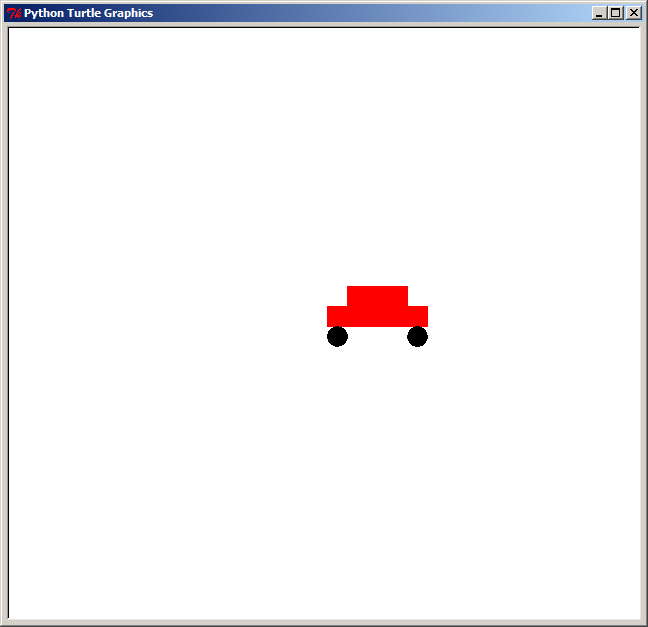
\includegraphics[scale=0.4]{images/voiture}
\caption{Voiture primitive}\label{fig:voiture}
\end{figure}

Néanmoins cet exemple montre quelques autres fonctions de « \texttt{turtle} »:
\begin{itemize}
\item « \texttt{color} » qui change la couleur du stylo;
\item « \texttt{begin\_fill} » et « \texttt{end\_fill} » pour remplir des zones;
\item et « \texttt{circle} » pour dessiner des cercles d'une taille donnée.
\end{itemize}


\section{Connaissez vous les couleurs?}

La fonction « \texttt{color} » prend trois paramètres. Le premier pour la quantité de rouge, le seconde pour la quantité de vert et le dernier pour la quantité de bleu.\\

\emph{Pourquoi rouge, vert et bleu?}\\


Si vous avez déjà joué avec différentes couleurs de peinture, vous connaissez déjà une partie de la réponse à cette question. Quand vous mélangez deux couleurs de peinture différentes vous obtenez une troisième couleur. En informatique les trois couleurs primaires sont rouge, vert et bleu. C'est à dire qu'à partir de ces trois couleurs on obtient toutes les couleurs qui peuvent être affichées sur l'écran\footnote{Pour la peinture, les trois couleurs primaires sont jaune, magenta, cyan.}. La \autoref{fig:r+v+b_bis} vous montre le principe de l'addition des couleurs.

\begin{figure}[h!]
\centering
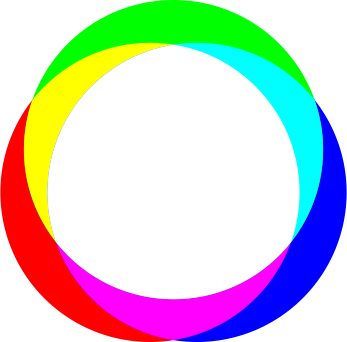
\includegraphics[scale=0.6]{images/r+v+b_bis}
\caption{Addition des couleurs primaires}\label{fig:r+v+b_bis}
\end{figure}

La lumière blanche est composée d'un mélange des différentes couleurs.
Chaque peinture crée de la couleur car elle absorbe certaines couleurs de la lumière blanche et ne laisse qu'une partie repartir. 
Quand vous mélangez des peintures, les différentes couleurs absorbées s'ajoutent. C'est pourquoi quand vous mélanger une peinture rouge et une peinture bleu vous avez du violet, plus foncé. De même si vous mélangez de nombreuses couleurs vous obtenez, habituellement, du brun boueux.
 
Sur un ordinateur, c'est un peu pareil mise à part que nous combinons des émissions de lumière. Si nous combinons du rouge et du bleu nous obtenons du magenta plus clair.
Nous avons trois projecteurs que nous pouvons régler de zéro à cent pourcent (en fait de 0 à 1).

La fonction « \texttt{color} » comme la plupart des fonctions manipulant les couleurs en informatique prend les couleurs dans l'ordre rouge, vert et bleu. Traçons maintenant un disque jaune:

\begin{Verbatim}[frame=single,rulecolor=\color{mbleu}, label=à taper]
tortue.color(1,1,0)
tortue.begin_fill()
tortue.circle(100)
tortue.end_fill()
\end{Verbatim}

Dans l'exemple ci-dessus, nous appelons la fonction « \texttt{color} » avec 100\% de rouge, 100\% de vert et 0\% de bleu (en d'autres termes 1, 1 et 0). Pour faire des expériences plus facilement avec différentes couleurs, transformons ce code en fonction:
\begin{Verbatim}[frame=single,rulecolor=\color{mbleu}, label=à taper]
def mondisque(rouge, vert, bleu):
    tortue.color(rouge, vert, bleu)
    tortue.begin_fill()
    tortue.circle(100)
    tortue.end_fill()
    
mondisque(0, 1, 0)
mondisque(0, 0.5, 0)
\end{Verbatim}

Nous pouvons tracer un disque vert vif avec « \texttt{mondisque(0, 1, 0)} »  en utilisant le projecteur vert réglé au maximum. Nous pouvons tracer un disque vert foncé avec « \texttt{mondisque(0, 0.5, 0)} » en utilisant le projecteur réglé à la moitié. Comme nous utilisons de la lumière, moins de couleur signifie généralement un résultat plus sombre. C'est comme avec une lampe torche: si la batterie est chargée vous avez une lumière claire qui devient de plus en plus sombre avec la décharge de la batterie.

De manière à le voir par vous même, essayez de tracer un cercle avec le rouge à fond puis à moitié (1 et 0,5), puis avec le bleu à fond puis à moitié.

\begin{Verbatim}[frame=single,rulecolor=\color{mbleu}, label=à taper]
mondisque(1, 0, 0)
mondisque(0.5, 0, 0)
mondisque(0, 0, 1)
mondisque(0, 0, 0.5)
\end{Verbatim}

Différentes combinaisons de rouge, de vert et de bleu produirons une grande variété de couleurs.
Vous pouvez avec une couleur orangée en utilisant 100\% de rouge, 85\% de vert et pas de bleu: « \texttt{mondisque(1, 0.85, 0)} ».

Une couleur rose bonbon peut être réalisée en combinant 100\% de rouge, 70\% de vert et 75\% de bleu: « \texttt{mondisque(1, 0.7, 0.75)} ». 

Vous aurez du orange en combinant 100\% de rouge et 65\% de vert. Le brun peut être obtenu en combinant 100\% de rouge, 30\% de vert et 15\% de bleu:
\begin{Verbatim}[frame=single,rulecolor=\color{mbleu}, label=à taper]
mondisque(1, 0.65, 0)
mondisque(0.6, 0.3, 0.15)
\end{Verbatim}

N'hésitez pas à expérimenter par vous même. 

Vous pouvez d'ailleurs utiliser « \texttt{tortue.clear()} » pour effacer ce qui a été tracé.


\section{Remplissage}
Vous avez probablement déjà compris que les fonctions « \texttt{begin\_fill} » et « \texttt{end\_fill} » signalaient le début et la fin du zone à remplir. Le remplissage ne s'effectue réellement qu'une fois que la commande « \texttt{end\_fill} » est invoquée et que Python peut déterminer avec exactitude la zone à remplir.

Premièrement, créons une fonction « \texttt{moncarré} »:
\begin{Verbatim}[frame=single,rulecolor=\color{mbleu}, label=à taper]
def moncarré(taille):
    for i in range(4):
        tortue.forward(taille)
        tortue.left(90)
\end{Verbatim}

Cette fonction dessine des carrés de taille variable selon votre choix.
Vous pouvez l'essayer avec plusieurs tailles:
\begin{Verbatim}[frame=single,rulecolor=\color{mbleu}, label=à taper]
moncarré(25)
moncarré(50)
moncarré(75)
moncarré(100)
\end{Verbatim}

Notre tortue devrait dessiner semblable à ce qui est présenté sur la \autoref{fig:4carrés}.

\begin{figure}[h!]
\centering
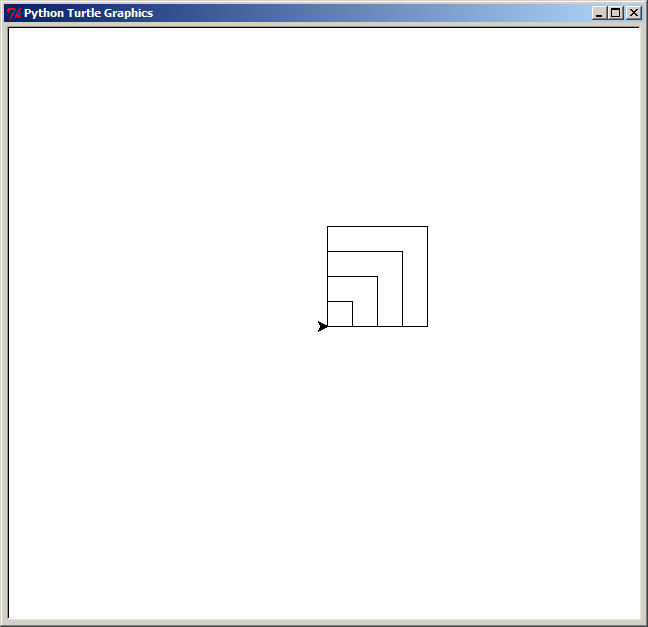
\includegraphics[scale=0.4]{images/4carres}
\caption{4 carrés}\label{fig:4carrés}
\end{figure}

Maintenant nous pouvons essayer un carré rempli. Premièrement nous allons commencer le remplissage avec
 « \texttt{begin\_fill} ». Puis nous l'arrêterons avec  « \texttt{end\_fill} ».

\begin{Verbatim}[frame=single,rulecolor=\color{mbleu}, label=à taper]
tortue.begin_fill()
moncarré(100)
tortue.end_fill()
\end{Verbatim}

Ce qui va produire un dessin comme le carré de la \autoref{fig:carrérempli}.
\begin{figure}[H]
\centering
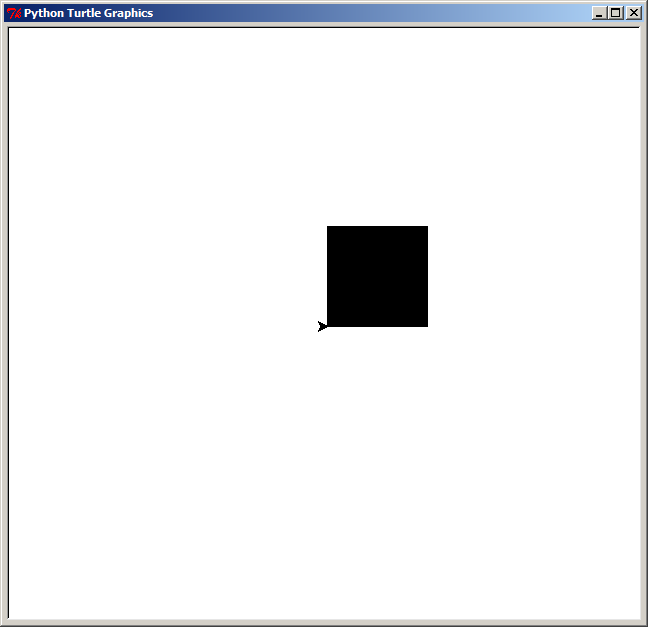
\includegraphics[scale=0.4]{images/carrerempli}
\caption{Un carré rempli}\label{fig:carrérempli}
\end{figure}

Comment changer la fonction de manière à ce que nous puisions dessiner un carré, rempli ou non? Nous avons besoin d'un autre paramètre, ce qui est légèrement plus compliqué de la manière suivante:

\begin{Verbatim}[frame=single,rulecolor=\color{mbleu}, label=à taper]
def moncarré(taille, rempli):
    if rempli == True:
        tortue.begin_fill()
    for i in range(4):
        tortue.forward(taille)
        tortue.left(90)
    if rempli == True:
        tortue.end_fill()
        
moncarré(50, True)
moncarré(150, False)
\end{Verbatim}

Dans les deux premières lignes de la fonction nous vérifions si le paramètre « \texttt{rempli} » vaut « \texttt{True} ». Si c'est le cas alors la fonction « \texttt{begin\_fill} »  est lancée. Nous bouclons alors quatre fois pour dessiner un carré avant de vérifier une seconde fois si le paramètre « \texttt{rempli} » vaut vrai.
Si cela est le cas nous lançons alors la fonction « \texttt{end\_fill} ».

Puis nous traçons un carré plein et un carré vide pour tracer l'image de la \autoref{fig:oeil}. Maintenant que j'y pense, elle ressemble à un drôle d'œil carré.

\begin{figure}[h!]
\centering
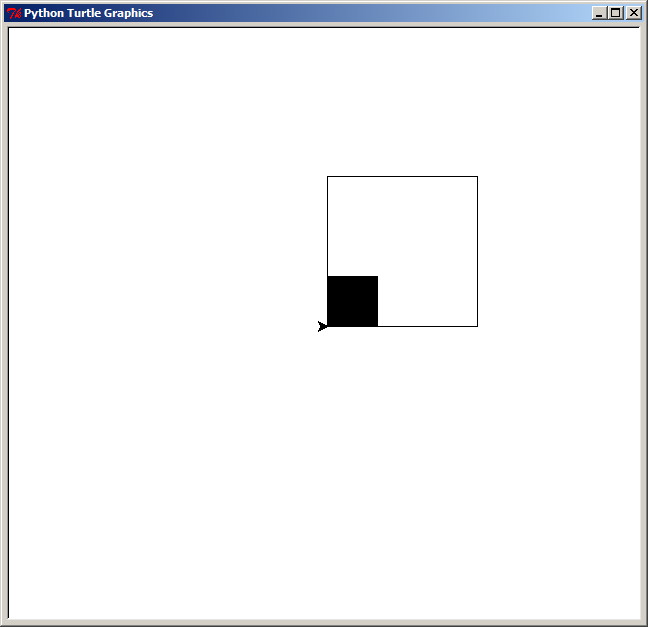
\includegraphics[scale=0.4]{images/oeil}
\caption{Œil fait avec des carrés}\label{fig:oeil}
\end{figure}

Vous pouvez dessiner toute sorte de formes et les remplir avec des couleurs. Revenons à une des étoiles que nous avions tracée plus tôt. Le code original ressemblait à cela:
\begin{Verbatim}[frame=single,rulecolor=\color{gray}, label=ne pas saisir]
for x in range(1,19):
    tortue.forward(100)
    if x % 2 == 0:
        tortue.left(175)
    else:
        tortue.left(225)
\end{Verbatim}

Nous pouvons utiliser les mêmes « tests si »  de la fonction « \texttt{moncarré} » et utiliser le paramètre de taille comme paramètre dans la fonction « \texttt{forward} ».

\begin{Verbatim}[frame=single,rulecolor=\color{mbleu}, label=à taper]
def monétoile(taille, rempli) :
    if rempli == True:
        tortue.begin_fill()
    for x in range(1,19):
        tortue.forward(taille)
        if x % 2 == 0:
            tortue.left(175)
        else:
            tortue.left(225)
    if rempli == True:
        tortue.end_fill()
\end{Verbatim}

À la deuxième et à la troisième ligne, nous contrôlons si le paramètre « \texttt{rempli} » vaut vrai, si c'est le cas nous activons le remplissage. Nous faisons similairement, à la dixième et onzième ligne, mais nous arrêtons la zone de remplissage, c'est à ce moment que le remplissage se fait.

L'autre différence à propos de cette fonction est que nous passons la taille de l'étoile (en fait d'une branche de l'étoile) comme paramètre et que nous utilisons cette valeur à la cinquième ligne.

Maintenant choisissons la couleur de l'étoile, par exemple orangé (vous vous rappelez peut-être qu'orangé est fait en mélangent 100\% de rouge, 85\% de vert et pas de bleu), puis appelons la fonction.

\begin{Verbatim}[frame=single,rulecolor=\color{mbleu}, label=à taper]
tortue.color(1, 0.85, 0)
monétoile(120, True)
\end{Verbatim}

La tortue devrait tracer l'étoile de la \autoref{fig:etoileorange}.
\begin{figure}[h!]
\centering
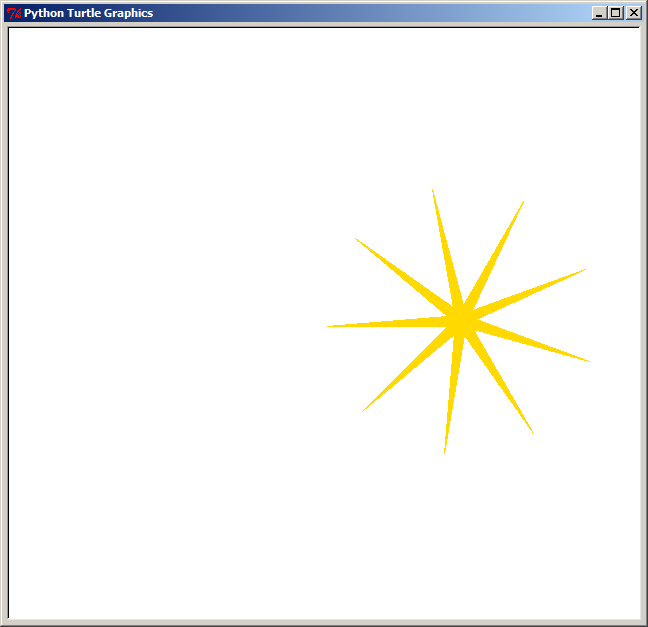
\includegraphics[scale=0.4]{images/etoileorange}
\caption{Étoile orangée simple}\label{fig:etoileorange}
\end{figure}

Nous pouvons ajouter un contour à l'étoile en changeant la couleur à nouveau (cette fois par exemple en noir) et redessiner en plus une étoile similaire mais sans remplissage.
\begin{Verbatim}[frame=single,rulecolor=\color{mbleu}, label=à taper]
tortue.color(0, 0, 0)
monétoile(120, False)
\end{Verbatim}

Cette fois-ci l'étoile ressemble à la \autoref{fig:etoileorange2}
\begin{figure}[h!]
\centering
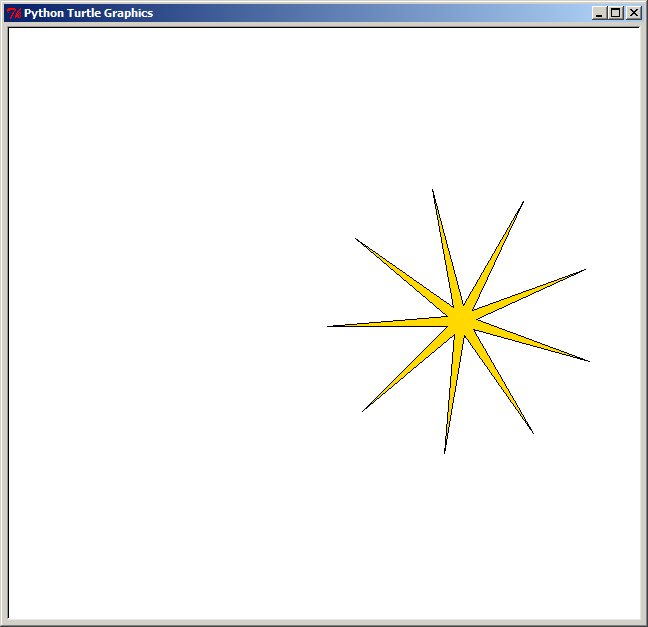
\includegraphics[scale=0.4]{images/etoileorange2}
\caption{Étoile orangée finalisée}\label{fig:etoileorange2}
\end{figure}

\section{Obscurité}

\emph{J'ai une question pour vous: qu'arrive-t'il quand vous éteignez toutes les lumières pendant la nuit?}\\

Tout devient noir. La même chose arrive avec les couleurs sur un ordinateur. Absence de couleur signifie absence de lumière. Ainsi la fonction « \texttt{mondisque} » avec les trois couleurs à zéro produit un disque noir. L'inverse est vrai aussi, si les trois couleurs sont à un, la couleur résultante est le blanc.

Pour faire un joli dessin, je me dois de vous informer que les fonctions peuvent prendre des paramètres optionnels. Des paramètres facultatifs qui, s'ils sont utilisés, modifient le résultat d'une fonction.

Par exemple la méthode « \texttt{circle} », en plus du rayon, peut prendre deux paramètres optionnels: l'angle « \texttt{extent} » (\emph{extent} signifie étendue en anglais) et le nombre d'étapes pour réaliser le tracé « \texttt{steps} »   (\emph{step} signifie étape en anglais).

La méthode circle s'utilise « \texttt{circle(rayon,angle,étapes)} », si aucun angle n'est fourni alors l'angle vaut 360 degrés (le cercle est complet). Si l'on choisi des angles plus petits des arcs de cercle seront tracés. Par exemple, 90 degrés permettront de faire de quarts de cercle et 180 degrés permettront de faire des demi-cercles.

Pour être exact \emph{on nous cache tout, on nous dit rien}\footnote{Chanson de Jacques Dutronc}, le rayon peut être choisi positif ou \emph{négatif}. Si le rayon est positif la tortue avance en tournant vers la gauche. Si le rayon est négatif la tortue avance en tournant vers la droite\footnote{Si vous n'avez pas encore vu les nombres négatifs ailleurs que sur un thermomètre, ce n'est pas grave retenez juste le changement de sens.}.

L'angle « \texttt{extent} » peut lui aussi être choisi négatif ou positif. Si l'angle est négatif la tortue va reculer au lieu d'avancer. Les paramètres optionnels peuvent facilement être utilisés dans l'ordre (c'est à dire les premiers mais pas les derniers). Faisons quelques tests:

\begin{Verbatim}[frame=single,rulecolor=\color{mbleu}, label=à taper]
tortue.circle(-100)
tortue.circle(100)
tortue.left(90)
tortue.circle(100, 90)
tortue.circle(100, -90)
tortue.right(90)
tortue.circle(100, -180)
tortue.right(90)
tortue.circle(-100, -90)
\end{Verbatim}

Vous devriez avoir un résultat similaire à celui de la \autoref{fig:baseball}.

\begin{figure}[H]
\centering
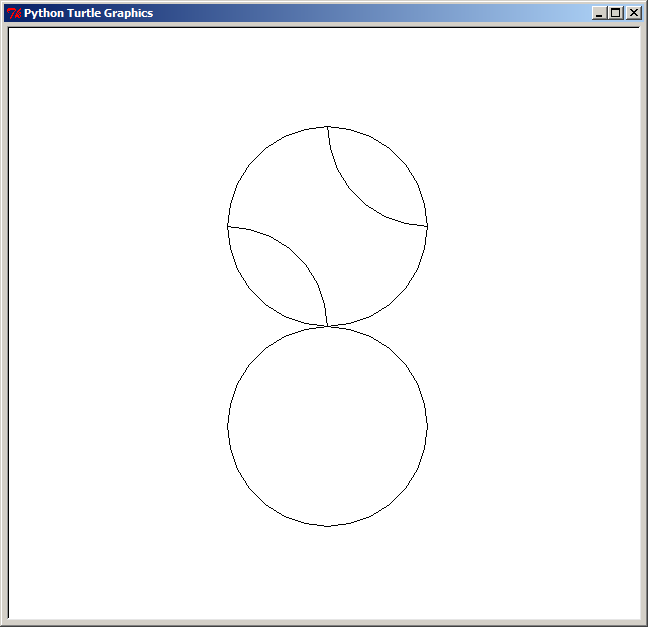
\includegraphics[scale=0.4]{images/baseball}
\caption{Tests avec les rayons et les arcs de cercle}\label{fig:baseball}
\end{figure}

Le nombre d'étapes est automatiquement déterminé sauf si on l'impose. Néanmoins il peut être utile de choisir des valeurs pour tracer des polygones réguliers. Il est possible de modifier un paramètre optionnel, sans modifier les autres, en le nommant. Attention le nombre d'étapes « \texttt{steps} » doit être strictement supérieur à zéro. La fonction « \texttt{circle} » réalise une division du cercle théorique par le nombre d'étapes pour trouver les sommets du polygone correspondant aux différentes étapes. Il se trouve que la division par zéro n'est pas une très bonne idée et n'a pas un résultat déterminé ce qui ne plaît pas trop aux ordinateurs en général et à Python en particulier.

\begin{Verbatim}[frame=single,rulecolor=\color{mbleu}, label=à taper]
for i in range(1,6):
	tortue.circle(100, steps=i)
\end{Verbatim}


La \autoref{fig:poly} montre le résultat de ces instructions. 
Comme vous pouvez le voir, le « cercle » en deux étapes est un segment qui est dessiné par un aller-retour avec un retour à la position de départ.
Le « cercle » en trois étapes est un triangle. Le « cercle » en quatre étapes est un carré et ainsi de suite. 
Rappelez-vous notre cercle fait avec un itérateur quand nous ne connaissions pas la fonction « \texttt{circle} ».
En fait, il s'agissait d'un cercle en 360 étapes. La fonction « \texttt{circle} » calcule automatiquement le nombre adéquat d'étapes pour que le cercle affiché ressemble vraiment à un cercle.

\begin{figure}[H]
\centering
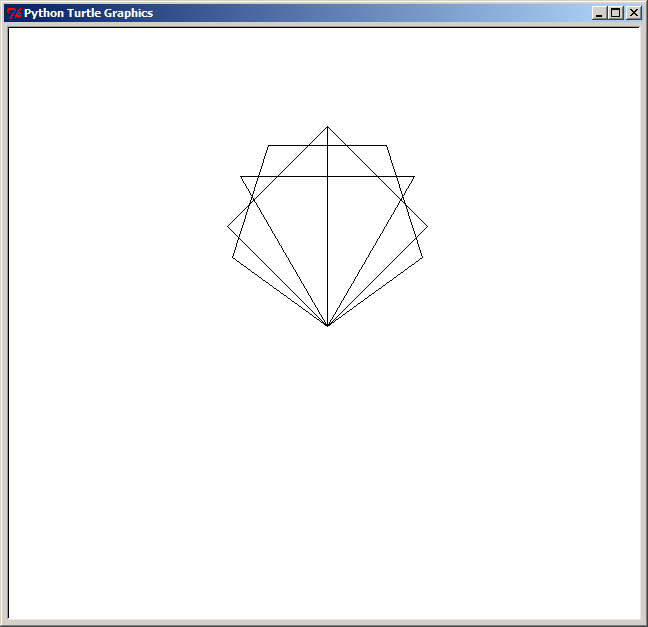
\includegraphics[scale=0.4]{images/poly}
\caption{Polygones obtenus grâce à « \texttt{circle} »}\label{fig:poly}
\end{figure}

%\clearpage{}
Nous pouvons aussi définir notre propre fonction avec des paramètres optionnels. En ajoutant, à coté du nom du paramètre, la valeur par défaut qui sera utilisée si aucune valeur n'est fournie.  Par exemple, « \texttt{def moncercle(rayon, angle=360, plein=False) :} » défini une fonction « \texttt{moncercle} »  dont l'angle est par défaut 360 degré comme sur la fonction « \texttt{circle} » mais qui peut être plein (par défaut) ou pas.


Nous allons maintenant tracer le symbole du Yin « {\fontspec{AR PL UMing CN}陰} »  et du Yang « {\fontspec{AR PL UMing CN}陽} ».

\begin{Verbatim}[frame=single,rulecolor=\color{mbleu}, label=à taper]
def moncercle(rayon, angle=360, plein=False) :
    if plein:
        tortue.begin_fill()
        tortue.circle(rayon, angle)
        tortue.end_fill()
    else :
        tortue.circle(rayon, angle)

tortue.color(0, 0, 0)
moncercle(100, 180, True)
moncercle(50, plein=True)
tortue.left(90)
tortue.forward(60)
tortue.left(90)
tortue.color(1, 1, 1)
moncercle(10, plein=True)
tortue.up()
tortue.right(90)
tortue.forward(40)
tortue.left(90)
tortue.down()
moncercle(-50, 180, True)
tortue.left(180)
tortue.color(0, 0, 0)
moncercle(100)
tortue.left(90)
tortue.up()
tortue.forward(60)
tortue.down()
tortue.left(90)
moncercle(10, plein=True)
\end{Verbatim}

Avec un peu de chance vous devriez obtenir le résultat de la \autoref{fig:yinyang}.

\begin{figure}[h!]
\centering
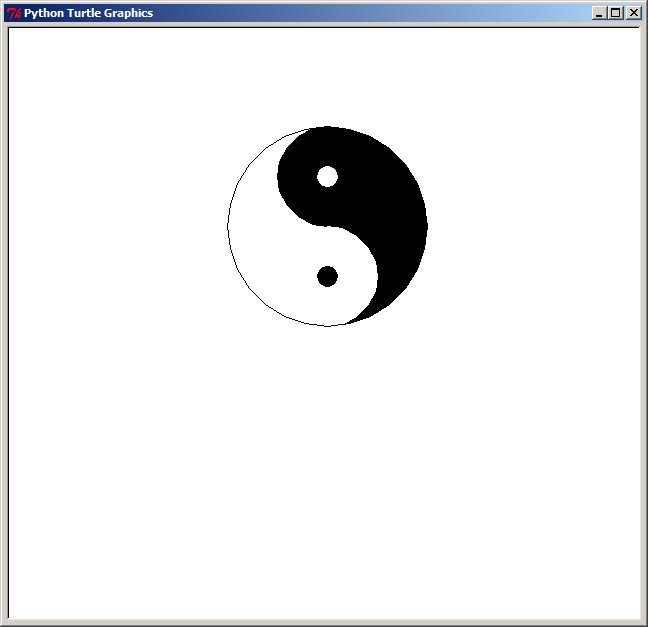
\includegraphics[scale=0.4]{images/yinyang}
\caption{Symbole du Yin et du Yang}\label{fig:yinyang}
\end{figure}

Vous pouvez sauvegarder le programme en utilisant l'extension de fichier « \texttt{.pyw} » (py comme PYthon et w comme Windows) sur le bureau typiquement. Si on exécute le programme en double cliquant dessus seul l'affichage de dessin se fera sans fenêtre texte derrière contrairement à ce qui ce passe avec l'extension « \texttt{.py} ». Par exemple j'ai appelé mon programme « \texttt{yinyang.pyw} ». Ce programme peut être exécuté sur tout ordinateur où Python est installé. Il est possible de convertir les programmes Python en exécutable avec « \texttt{py2exe} » mais cela n'est pas expliqué dans ce livre car cela nécessite l'installation d'un logiciel supplémentaire\footnote{Py2exe est un logiciel libre téléchargeable sur le site \url{http://www.py2exe.org/}.}.


\section{À vous de jouer\label{PRATIQUE:PROFUSION}}

Dans ce chapitre nous avons complété nos connaissances du module « \texttt{turtle} » et nous l'avons utilisé pour tracer des figures plus complexes. Nous avons utilisé des fonctions de manière à réutiliser notre code et en particulier pour tracer des dessins de couleurs différentes.

Vous trouverez des pistes de réponses dans la \autoref{REPONSES:PROFUSION}.


\subsection{Exercice 1}
Nous avons tracé des étoiles, des carrés et des cercles. Pouvez-vous tracer un octogone régulier? Un octogone est une forme (un polygone) à huit cotés. Un octogone régulier a tous ses cotés égaux ainsi que tous ses angles aux sommets.

Indice: 360 divisés par 8 font 45, un octogone est plus proche d'un cercle qu'un carré.

\subsection{Exercice 2}
Maintenant convertissez le code pour dessiner un octogone en une fonction qui permet de créer un octogone rempli avec une couleur.


 \vfill
\begin{center}
 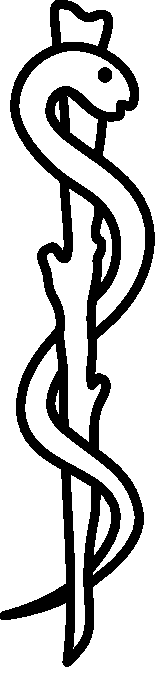
\includegraphics[width=2cm]{images/Esclapius_stick.pdf}
\end{center}
 \vfill

